\documentclass[a4paper]{scrreprt}

\usepackage[ngerman]{babel}
\usepackage[utf8]{inputenc}
\usepackage[T1]{fontenc}
\usepackage{ae}
\usepackage[bookmarks,bookmarksnumbered]{hyperref}
\usepackage{tabularx}
\usepackage{graphicx}


\newenvironment{requirement}[5] {
	\subsection{#1}
	\begin{tabularx}{\textwidth}{|X|l|X|X|}
		\hline
		Priorität & Zuständiger & Arbeitsaufwand & Abhängigkeiten \\
		\hline
		#2 & #3 & #4 & #5 \\
		\hline
	\end{tabularx}
	}{
	\newpage
	}


\begin{document}

% Title page
\title{Pflichtenheft}
\author{
	Bayram, Burak
	\and
	Kirsch, Julian
	\and
	Lang, Linda
	\and
	Schott, Erik
	\and
	Weggel, Tom
}
\maketitle

\newpage

% TOC
\tableofcontents
\newpage

% Intro
\chapter{Einleitung}
\section{Zweck und Ziel dieses Dokuments}

Dieses Dokument dient dem Projektmanagement. Gemäß der Art eines Pflichtenhefts bestimmt dieses Dokument Ziele sowie die Wichtigkeit der Ziele, also ob das Ziel ein Muss-, ein Soll- oder ein Kann-Ziel ist. Des Weiteren werden die Ziele in Meilensteine gruppiert.

Jedes Ziel wurde mit dem gleichen Aufbau formuliert. Dazu wird eine Tabelle angeführt, welche Priorität, Abhängigkeiten von anderen Zielen, Zuständigkeiten und eine geschätzte Bearbeitungsdauer für jedes Ziel enthält.
Weiterhin besteht jedes Ziel aus einer Beschreibung, welche mit einer sogenannten User Story angeführt wird.


\section{Ziel und Zweck des Projektes}

Ziel dieses Projektes ist es einen Client zu einem gegebenem Server zu implementieren, welcher selber das Brettspiel \glqq Kingdom Builder\grqq{} implementiert.

Ein Client kann eigene Spiele erstellen und verwalten oder einem bereits erstelltem Spiel beitreten. Spiele können hierbei lokal im sog. \glqq Hot-Seat\grqq{}-Modus
oder über das Netzwerk gegen andere Spieler oder Bots gespielt werden.

\section{Nicht-Ziele des Projektes}

Ziel des Projektes ist \textbf{nicht} die Implementierung eines Spieleservers.

\section{Einsatz und Umgebung}

Das Produkt ist für Endverbraucher geeignet, die einen Computer besitzen. Des Weiteren ist für die Inbetriebnahme eine Installation der \glqq Java Runtime Environment 17\grqq{} (oder neuer) erforderlich.

Für die Onlinefunktionalität wird eine Internetverbindung benötigt.

\section{Projektorganisation}
\subsection{Meilensteine}

Die Entwicklung des Projektes wird in Meilensteinen unterteilt. Dabei verfolgen die Meilensteine aufeinander aufbauende Ziele.

Der erste Meilenstein \glqq Chat Client\grqq{} dient der Umsetzung eines grundlegendes Systems, das ermöglicht einen Client bei dem Server zu registrieren und die dortigen Chatfunktionen zu nutzen.

Der zweite Meilenstein \glqq Basis Spiel\grqq{} umfasst die Implementierung des Basisspiels, sodass Spieler eine Lobby erstellen oder einer bestehenden Lobby beitreten
können und das Spiel gemäß der Regeln spielen können. Es wird erwartet, dass alle grundlegenden Eigenschaften umgesetzt werden. Dies umfasst sowohl die grafische Darstellung des Spiels als auch die Implementierung aller erforderlichen Spielregeln.

Der dritte und letzte Meilensteine \glqq KI\grqq{} sieht vor, dass eine künstliche Intelligenz entwickelt wird gegen die Spieler spielen können. Des Weiteren ist auch ein \glqq Hot-Seat\grqq{}-Modus vorgesehen, welcher es ermöglicht mehreren Spielern gemeinsam an einem Computer zu spielen.

\subsection{Entwicklerrollen}

Innerhalb des Projektes nimmt jeder Teilnehmer eine spezifische Rolle an und ist somit Verantwortlicher und Ansprechpartner für einen Teilbereich des Projektes:

\begin{description}
	\item[Build-Master (Julian Kirsch)] ist verantwortlich für das Einrichten, Verwalten und Pflegen des Gradle Projekts.
						 Diese Person sorgt dafür, dass das gesamte Projekt mittels Gradle gebaut werden kann.
						 Ansprechpartner für alles, was mit den Bauen des Projektes zu tun hat.
	\item[Design-Pattern-Master (Linda Lang)] hat die Aufgabe den Einsatz von Entwursmustern an allen Teilen des Projektes zu prüfen und den jeweiligen Modul-Mitgliedern bei der
							    Umsetzung zu helfen.
	\item[Dokumentation-Master (Tom Weggel)] ist dafür verantwortlich, dass alle relevanten (insbesondere alle sichtbaren) Methoden, Funktionen, Konstanten, etc. mittels JavaDoc
							       dokumentiert  werden und diese auf dem neuesten Stand sind.
	\item[Interface-Master (Erik Schott)] ist für die Schnittstellen zwischen den einzelnen Module verantwortlich und klärt Anforderungen, Umfang und Funktion der einzelnen Komponenten
						      des Softwareprojekts.
	\item[Test-Master (Burak Bayram)] entscheidet was getestet werden soll und sorgt dafür, dass die Tests geschrieben werden.
\end{description}

\subsection{Benutzerrollen}

Dieses Dokument beschreibt Ziele anhand von drei Benutzerrollen. Erstere ist die Rolle des \textbf{Spielers}, welcher, wie der Name schon andeutet, der Konsument des Spiels ist und mit dem
Produkt interagiert.

Die zweite Rolle, nämlich der \textbf{Root Spieler} (kurz: Root), bezieht sich auf Spieler, welche einen eigenen Spieleserver betreiben. Im Gegensatz zu normalen Spielern hat der Root administrative Freigaben und kann bspw. Spieler vom Server \glqq kicken\grqq{}.

Zuletzt gibt es die Rolle des \textbf{Entwicklers}, welcher aktiv das hier spezifizierte Produkt entwickelt.

\subsection{Arbeitsweise}
Im Folgenden sind Arbeitsweisen festgelegt, die für alle teilnehmende Entwickler verpflichtend sind.

\subsubsection{Branches}
Zu jedem Zeitpunkt im Projekt existieren zwei Branches, nämlich \glqq master\grqq{} sowie \glqq development\grqq{}. Der master-Branch stellt den aktuellsten Zustand des Projektes \textbf{nach} Abschließen eines Meilensteins dar. Der development-Branch hingegen spiegelt den aktuellsten Entwicklungsstand wider.

Des Weiteren soll, sofern semantisch sinnvoll, für jedes Ziel, das bearbeitet wird, ein eigener, sog. \glqq Feature-\grqq{}Branch erstellt werden.

Die Branches werden der \glqq GitFlow\grqq{}-Methode folgend benannt.

\subsubsection{Pull Requests}
Ist die Entwicklung eines Zieles abgeschlossen, so muss ein \glqq Pull Request\grqq{} angelegt und von den jeweiligen Test- sowie Dokumentation-Master auf Vollständigkeit geprüft.

\subsubsection{Code Style}
Der Code Style ist strikt an den Java Konventionen gehalten. Die GUI-Elemente werden der SnakeCase-Konvention folgenden notiert und mit einem FXML-Tag versehen.

Des Weiteren muss folgende Reihenfolge der Elemente innerhalb einer Klasse eingehalten werden:
\begin{itemize}
	\item Statische Variablen
	\item Instanzvariablen
	\item Konstruktoren
	\item Methoden
	\item Setter
	\item Getter
\end{itemize}

\subsubsection{Unit Test Style}
Unit Tests werden pro Klasse mit JUnit 5 durchgeführt, wobei einzelne Testklassen, soweit es möglich ist, unabhängig voneinander sein müssen, damit fehlgeschlagene Tests eindeutig einer Klasse zugeordnet werden können.

Objekte aus anderen Klassen, die zum Testen benötigt werden als Member innerhalb der Testklasse aufgeführt und mittels einer Methode, die mit \glqq@BeforeEach\grqq{} annotiert ist, instanziiert.

Es müssen alle Methoden außer \glqq Getter\grqq{} und \glqq Setter\grqq{} getestet werden.

Wenn in einer Testmethode mehrere Assertions vorhanden sind, müssen diese mit der überladenen Funktion auch eindeutig benannt werden, damit bei einem fehlgeschlagenen Test auf eine Assertion zurückgeführt werden kann. Darüber hinaus sollen mehrere Assertions nur dann verwendet werden, wenn diese alle im gleichen Kontext stehen bzw. auf die selbe Art und Weise getestet werden.

Testklassen werden mit \glqq[KlassenName]Test\grqq{} und Testmethoden mit \\ \glqq test[FeatureName][optionalerSpezialFall]\grqq{} benannt.





\chapter{Ziele}
\section{Meilenstein: Chat Client}


\begin{requirement}{Grundaufbau der Programmarchitektur}{Hoch}{JK}{2h}{}

\begin{center}
	Als Entwickler möchte ich einen Grundlage für das Programm schaffen.
\end{center}

Hierbei soll eine Software-Komponente entwickelt werden, welche das Redux-Architekturmuster, samt \glqq Store\grqq{}, \glqq State\grqq{}, \glqq Reducer\grqq{} und \glqq Actions\grqq{} umsetzt. Diese Software-Komponente fungiert als Kern der Anwendung und stellt auch die Schnittstelle zwischen den verschiedenen Komponenten der Software dar.

\end{requirement}


\begin{requirement}{Spielerliste}{Hoch}{ES, TW}{4h}{2.1.6; 2.1.1}

\begin{center}
Als Spieler möchte ich mir andere Spieler anzeigen lassen, die mit dem Server verbunden sind.
\end{center}

Hierbei muss eine GUI-Komponente erstellt werden, welche alle aktuell mit dem Server verbundenen Spieler auflistet.

Durch eine Markierung in der Auflistung müssen Spieler für eine Direktnachricht auswählbar sein. Des Weiteren muss ein Button zur Verfügung stehen, welcher die Markierung wieder aufhebt.

\end{requirement}


\begin{requirement}{Chat-Log}{Hoch}{ES, TW}{20h}{2.1.6}

\begin{center}
Als Spieler möchte ich mit anderen Clients per Textnachricht kommunizieren und diese angezeigt bekommen.
\end{center}

Hierbei muss eine GUI-Komponente implementiert werden, welche ein- und ausgehende Nachrichten in chronologischer Reihenfolge anzeigt.

Des Weiteren muss das Versenden von lokalen Nachrichten, sofern der Spieler einem Spiel beigetreten ist, an eine Lobby, sowie das Versenden von direkt adressierten und \glqq globalen\grqq{} Nachrichten an alle Spielern auf den Server ermöglicht werden.

Nachrichten müssen visuell in sofern von einander differenziert werden, so dass...
\begin{itemize}
	\item ...Sender- bzw. Empfängernamen \textbf{fett} angezeigt werden.
	\item ...Nachrichten je nach Art (zum Beispiel Textnachricht oder Statusnachricht) farblich gekennzeichnet sind.
\end{itemize}
\end{requirement}


\begin{requirement}{Chat-Eingabe}{Hoch}{ES, TW, BB}{5h}{2.1.6}

\begin{center}
	Als Spieler möchte ich Textnachrichten für den Chat verfassen, um mit anderen Spielern zu kommunizieren.
\end{center}

Eine GUI-Komponente muss implementiert werden, die es ermöglicht Spieler per Tastatureingabe Text einzutippen. Weiter muss über Buttons die verfasste Nachricht \glqq global\grqq{} also serverweit/lobbyweit als auch an ausgewählte Spieler versendbar sein.

\end{requirement}


\begin{requirement}{Anzeigen von Statusnachrichten}{Mittel}{ES, TW}{3h}{2.6.1}

\begin{center}
	Als Spieler möchte ich benachrichtigt werden, wenn ich oder ein anderer Spieler den Server verlässt.
\end{center}

Hierbei muss der Chat-Log erweitert werden, so dass Statusnachrichten angezeigt werden.

\end{requirement}


\begin{requirement}{Spielprotokoll De-/Serialisieren}{Hoch}{JK}{20h}{-}

\begin{center}
	Als Entwickler möchte ich Nachrichten de-/serialisieren um mit denen Programmieren zu können.
\end{center}

Hierbei muss eine Software-Komponente entwickelt werden, welche Nachrichten vom Server in eine Objektpräsentation und Befehle an den Server von der Objektpräsentation in Textform
überführt. Hierfür müssen Nachrichten bzw. Befehle für folgende Aktionen oder Ereignisse unterstützt werden:
\begin{itemize}
	\item Ein- und Ausloggen des Spielers
	\item Abfrage der aktuellen Spieler
	\item Benachrichtigung über Beitritt/Verlassen eines Spielers
	\item Versenden einer Nachricht
	\item Empfangen einer Nachricht
\end{itemize}
\end{requirement}


\begin{requirement}{Verbindungsaufbau}{Hoch}{JK}{5h}{-}

\begin{center}
	Als Entwickler möchte ich eine Verbindung zu einem Spieleserver aufbauen, um Befehle zu versenden, Benachrichtigungen empfangen und auf diese reagieren zu können.
\end{center}

Hierbei muss eine Software-Komponente entwickelt werden, welche eine aktive Netzwerkverbindung aufbaut.

\end{requirement}


\begin{requirement}{Namenseingabe}{Hoch}{ES, TW}{1h}{2.1.1; 2.6.1}

\begin{center}
	Als Spieler möchte ich meinen eigenen Namen auswählen, der anderen Spielern angezeigt wird.
\end{center}

Hierbei muss eine GUI-Komponente erstellt sowie die Netzwerk-Komponente erweitert werden, so dass ein Nutzer seinen Wunschnamen angeben und sich auf dem Server einloggen kann.

\end{requirement}


\begin{requirement}{Verbindung beenden}{Hoch}{Julian Kirsch}{3h}{2.6.1}

\begin{center}
	Als Entwickler möchte ich eine bestehende Verbindung zum Server trennen um entweder das Programm zu beenden oder um auf andere Server beitreten zu können.
\end{center}

Hierbei muss die Netzwerk-Komponente erweitert werden, so dass diese den aktuellen Spieler vom Server ausloggt und die Verbindung schließt.

\end{requirement}


\section{Meilenstein: Basis Spiel}


\begin{requirement}{Hauptmenü-Maske (MainView)}{Hoch}{TW}{2h}{-}

\begin{center}
	Als Spieler möchte ich die Möglichkeit haben ein lokales Spiel zu starten, mich mit einem Spieleserver zu verbinden und die Programmeinstellungen zu ändern.
\end{center}


Hierbei muss eine GUI-Maske entworfen und implementiert werden, die folgende Buttons zur Verfügung stellen muss:
\begin{description}
	\item[Local Game] öffnet die Maske zum Erstellen eines Spiels (\glqq GameSettingsView\grqq{}).
	\item[Online Game] öffnet die Maske zur Initiierung einer neuen Netzwerkverbindung (\glqq ServerConnectView\grqq{}), sofern man nicht schon verbunden ist.
				Ansonsten wird direkt die Maske mit dem Spielbrowser (\glqq GameBrowserView\grqq{}) geöffnet.
	\item[Settings] öffnet die Einstellungs-Maske (\glqq ApplicationSettingsView\grqq{}).
	\item[Exit] beendet das Programm.
\end{description}

\begin{center}
	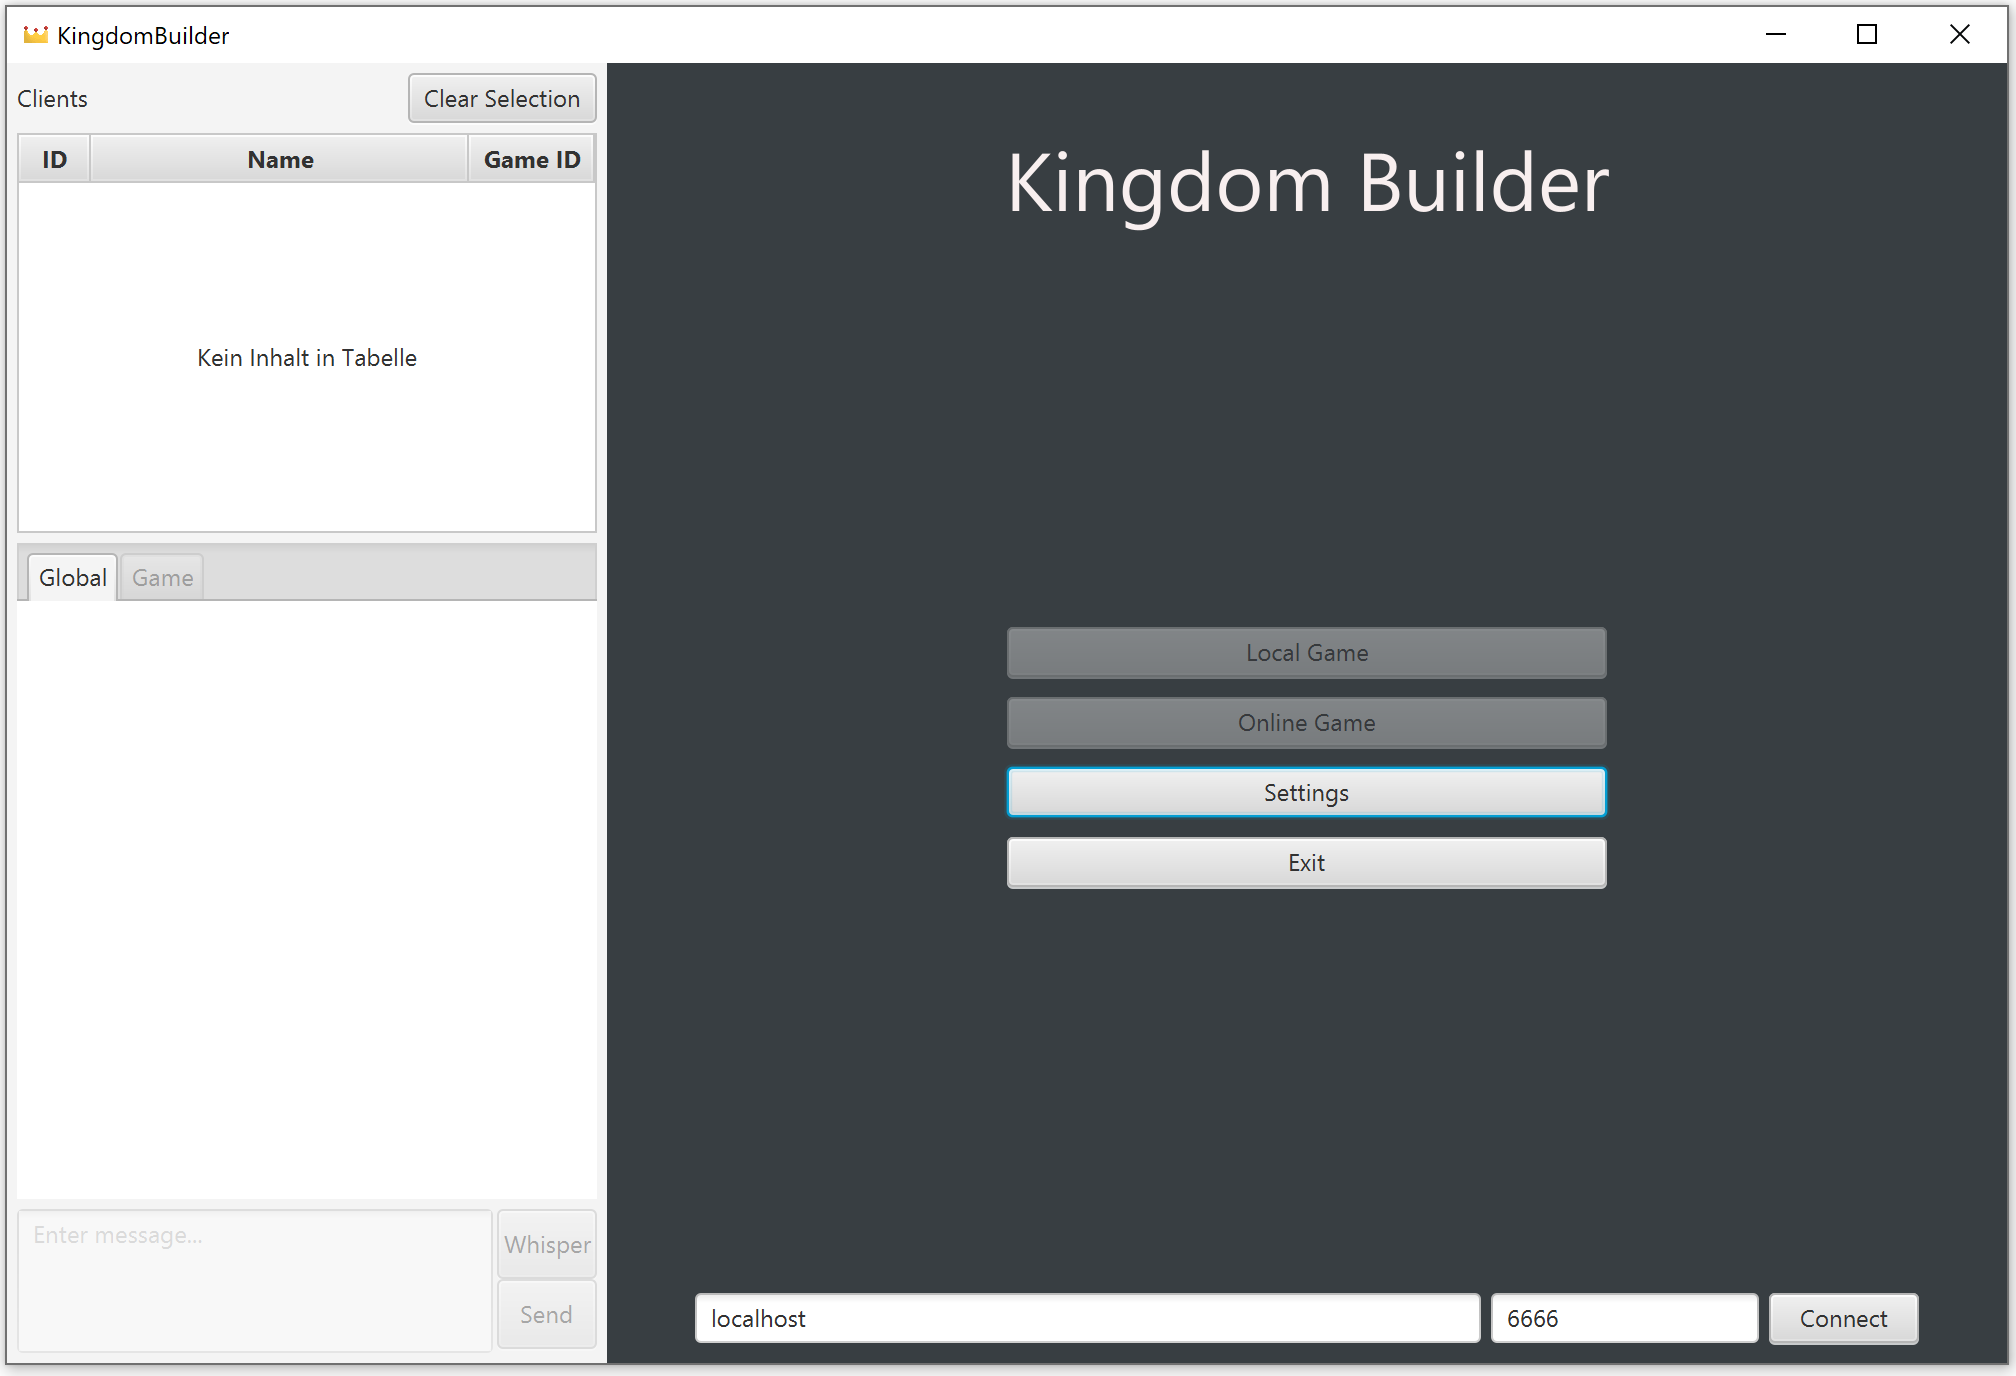
\includegraphics[width=0.8\textwidth]{view2.png}
	\\
	\tiny{(Skizze)}
\end{center}

\end{requirement}


\begin{requirement}{Einstellungs-Maske (ApplicationSettingsView)}{Mittel}{TW}{5h}{-}

\begin{center}
	Als Spieler möchte ich die Möglichkeit haben die Einstellungen des Programms zu ändern, um dieses an meine Anforderungen anzupassen.
\end{center}

Hierbei muss eine GUI-Maske entworfen und implementiert werden, die es einem ermöglicht die Präferenz aus einer Auswahl von verfügbaren Sprachen sowie den eigenen bevorzugten Namen zu setzen. Des Weiteren müssen zwei Buttons zur Verfügung gestellt werden, welche es ermöglichen die Änderungen anzuwenden oder direkt in die Hauptmenü-Maske \glqq MainView\grqq{} zu wechseln.

\end{requirement}


\begin{requirement}{Verbindungs-Maske (ServerConnectView)}{Hoch}{TW}{2h}{-}

\begin{center}
	Als Spieler möchte ich mich unter Angabe einer IP-Adresse zu einem Spieleserver verbinden.
\end{center}

Hierbei muss eine GUI-Maske entworfen und implementiert werden, die einem die Eingabe einer IP-Adresse ermöglicht. Weiter sollen auch zwei Buttons \glqq Verbinden \grqq{} und \glqq Zurück \grqq{} zur Verfügung stehen.

Wird der Button \glqq Verbinden\grqq{} geklickt, so wird eine Verbindung erstellt und der Nutzer zum Gamebrowser (\glqq GameBrowserView\grqq{})  geführt. Schlägt die Verbindung fehl, so wird der Nutzer über einen Dialog über den Fehler informiert.
Wird der Button \glqq Zurück\grqq{} geklickt, so wird der Nutzer zurück zum Hauptmenü (\glqq MainView\grqq{}) geführt.

\end{requirement}



\begin{requirement}{Gamebrowser (GameBrowserView)}{Hoch}{LL, TW}{7h}{-}

\begin{center}
	Als Spieler möchte ich ein Spiel erstellen, beobachten oder einem Spiel beitreten.
\end{center}

Hierbei muss eine GUI-Maske entworfen und implementiert werden, die alle Spiele des aktuellen Servers auflistet, sowie einem Spieler ermöglicht ein Spiel zu erstellen.

Es werden alle aktuell laufenden Spiele auf dem Server, zu dem der Client verbunden ist, angezeigt. Diesen Spielen kann als Spieler beigetreten werden, wenn sie nicht bereits voll besetzt sind. Es kann stets einem Spiel als Zuschauer beigetreten werden. Es kann außerdem ein neues Spiel erstellt werden.

In der oberen linken Ecke befinden sich 3 Buttons. Der erste Button \glqq Zurück \grqq{} sorgt dafür, zurück in das Hauptmenü (\glqq MainView \grqq{}) zu kommen.
Daneben befindet sich ein Button \glqq Refresh \grqq{}, um die Tabelle manuell zu aktualisieren.
Hierneben ist eine ComboBox, mit der man in der Tabelle nach einem gewissen Spiel-Zustand filtern kann. Nach der Auswahl in der Combobox wird die Tabelle anhand dieser angepasst.
Die laufenden Spiele werden in einer TableView angezeigt. Diese besitzt eine Spalte für den Namen des Spiels, die Anzahl der Spieler und den Status, ob das Spiel auf Spieler wartet, läuft oder beendet ist.

Auf der rechten Seite werden detaillierte Informationen zu dem in der Tabelle ausgewählten Spiel angezeigt. Diese Informationen bestehen aus dem Namen des Spiels, wer der Host des Spiels ist, dem eingestelltem Zeit- und Zuglimit. Anschließend folgt eine TextArea, die die Beschreibung des Spiels anzeigt.
Die Informationen werden mit einer GridPane gegliedert.

In der untersten Zeile befinden sich drei Buttons.
Der erste Button sorgt dafür, dass ein User ein Spiel erstellt und die View zu den Spiel-Settings wechselt.
Mit dem Button daneben betritt der User das in der Tabelle ausgewählte Spiel. Die aktuelle View wird zur View geändert, die das Spiel anzeigt.
Der letzte Button sorgt dafür, dass der User dem in der Tabelle ausgewählten Spiel als Zuschauer beitritt. Hierbei wird die View auch zur View geändert, die das Spiel anzeigt.

\begin{center}
	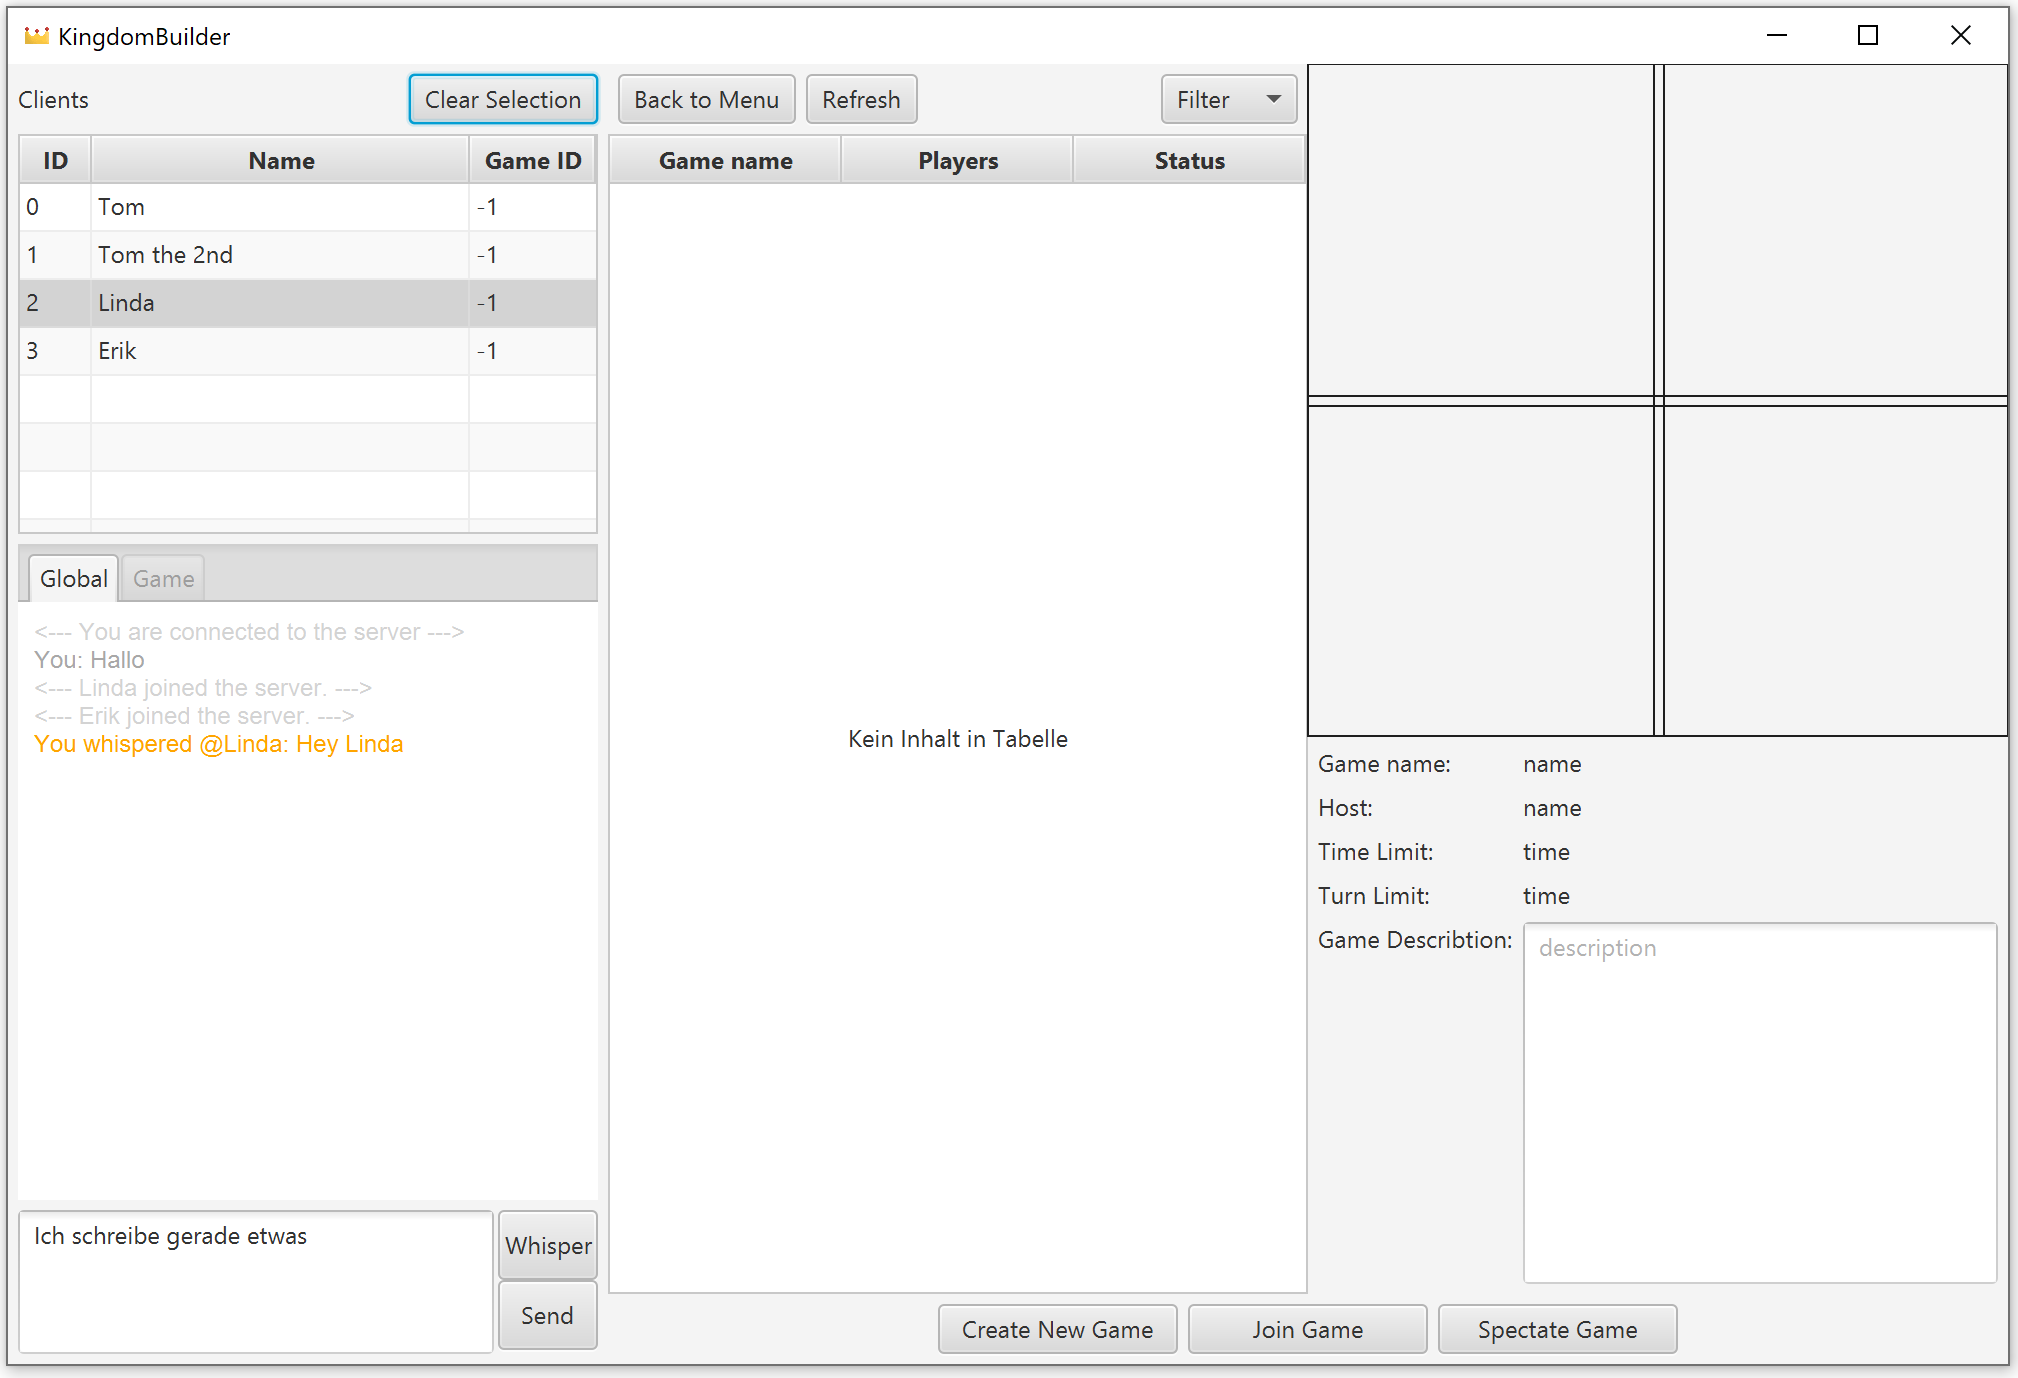
\includegraphics[width=0.8\textwidth]{view3.png}
	\\
	\tiny{(Skizze)}
\end{center}

\end{requirement}


\begin{requirement}{Spieleinstellungen (GameSettingsView)}{Hoch}{BB, TW, LL}{3h}{-}

\begin{center}
	Als Spieler möchte ich die Einstellungen für Spiel an meine Wünsche anpassen.
\end{center}

Hierbei soll eine GUI-Maske entworfen und implementiert werden, die einem Spieler ermöglichen folgende Einstellungen zu setzen:

\begin{itemize}
	\item Zeitlimit
	\item Zuglimit
	\item Maximale Spielerzahl
	\item Bots
\end{itemize}

Des Weiteren müssen Buttons angeboten werden, die einem ermöglichen das Spiel zu \glqq hosten\grqq{} und die Spieleinstellungen zu verlassen.
Wird der Button \glqq
Hosten\grqq{} geklickt, so wird das Spiel erstellt und der Ersteller tritt automatisch bei. Anschließend wird der Spieler in die Spielinformations-Maske (\glqq GameInfoView\grqq{}) geführt. Wird der Button \glqq Zurück\grqq{} gedrückt, so wird der Spieler zurück in das Hauptmenü (\glqq MainView\grqq{}) geführt.

\begin{center}
	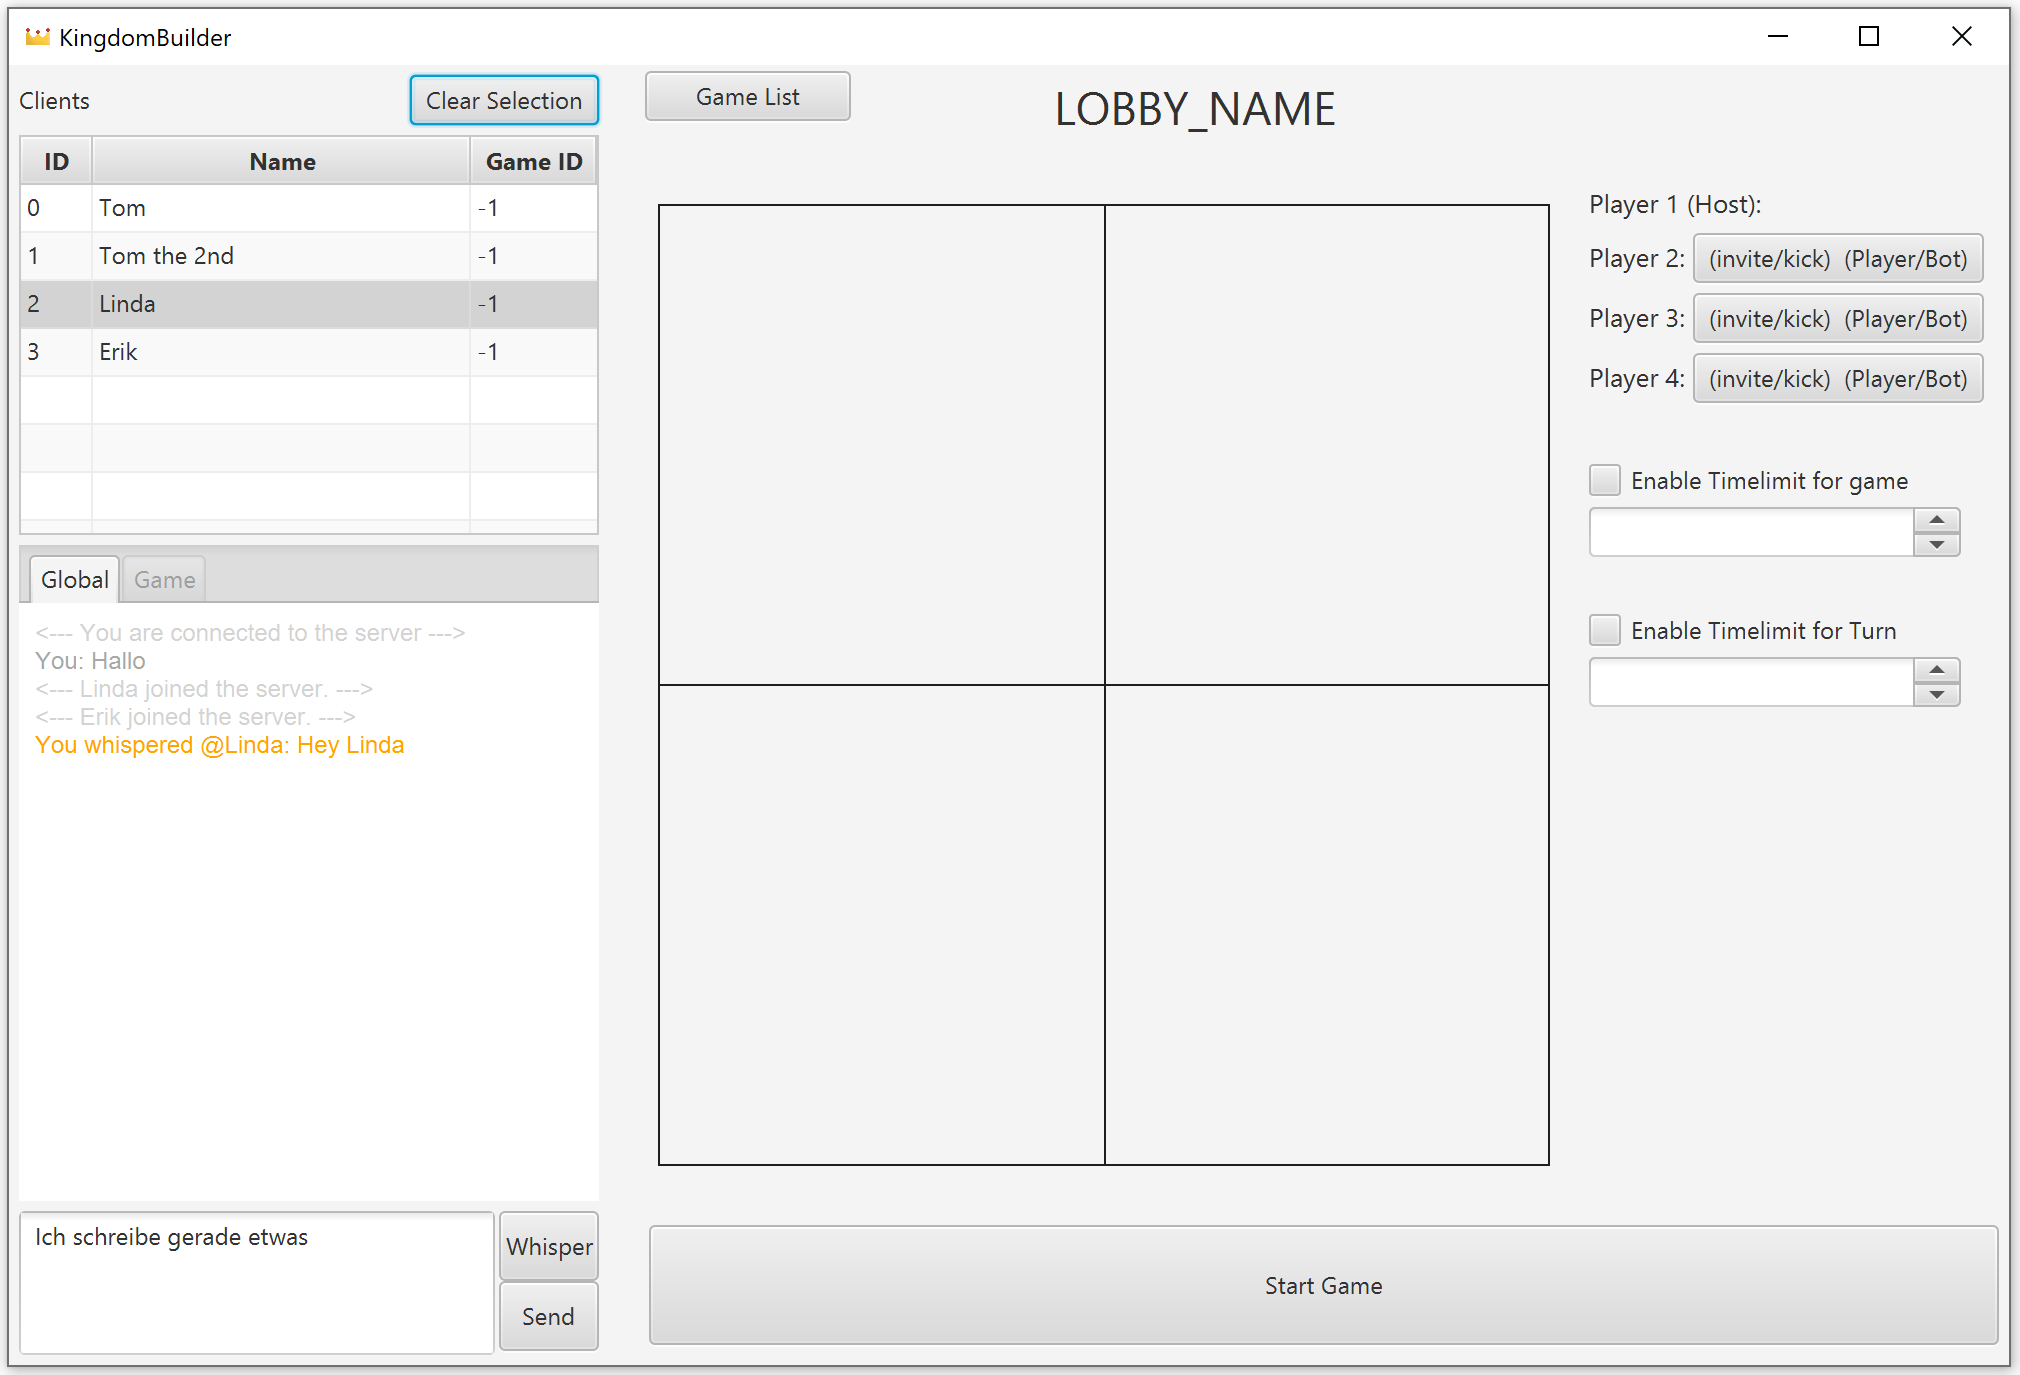
\includegraphics[width=0.8\textwidth]{view4.png}
	\\
	\tiny{(Skizze)}
\end{center}

\end{requirement}


\begin{requirement}{Spielinformationen (GameInfoView)}{Hoch}{TW}{6h}{-}

\begin{center}
	Als Spieler möchte ich Information über das aktuell beigetretene Spiel einsehen.
\end{center}

Hierbei muss eine GUI-Maske entworfen und implementiert werden, welche relevante Informationen über das aktuelle Spiel anzeigt.

Diese werden in zwei Bereiche unterteilt. Zunächst werden folgende Informationen angezeigt:
\begin{itemize}
	\item Anzahl der vergangenen Züge
	\item Zeitlimit
	\item Zuglimit
	\item Siegbedingung
	\item Spielerinformationen (Name, verbleibende Siedlungen, Punkte, Farbe)
\end{itemize}

Außerdem soll das Spielfeld, die Tokens und Anzahl der auswählbaren Hexagone angezeigt werden.

\end{requirement}



\begin{requirement}{Spielbrett (GameView)}{Hoch}{TW, LL}{30h}{2.2.6}

\begin{center}
	Als Spieler möchte ich das Spielbrett visuell dargestellt bekommen.
\end{center}

Hierbei muss eine GUI-Komponente dargestellt werden, welche alle Hexagone gemäß dem aktuellen Spielfortschitts darstellt. Des Weiteren müssen Interaktionen implementiert werden,
so dass die Karte bewegt und vergrößert sowie verkleinert werden kann. Es gilt zu beachten, dass Spieler die Karte nicht über den Rand hinaus bewegen dürfen sowie das Grenzen für das Verkleinern und Vergrößern der Karte gesetzt werden.

Die Karte muss über die Pfeiltasten bewegbar sein und über das Mausrad vergrößert oder verkleinert werden können.

\begin{center}
	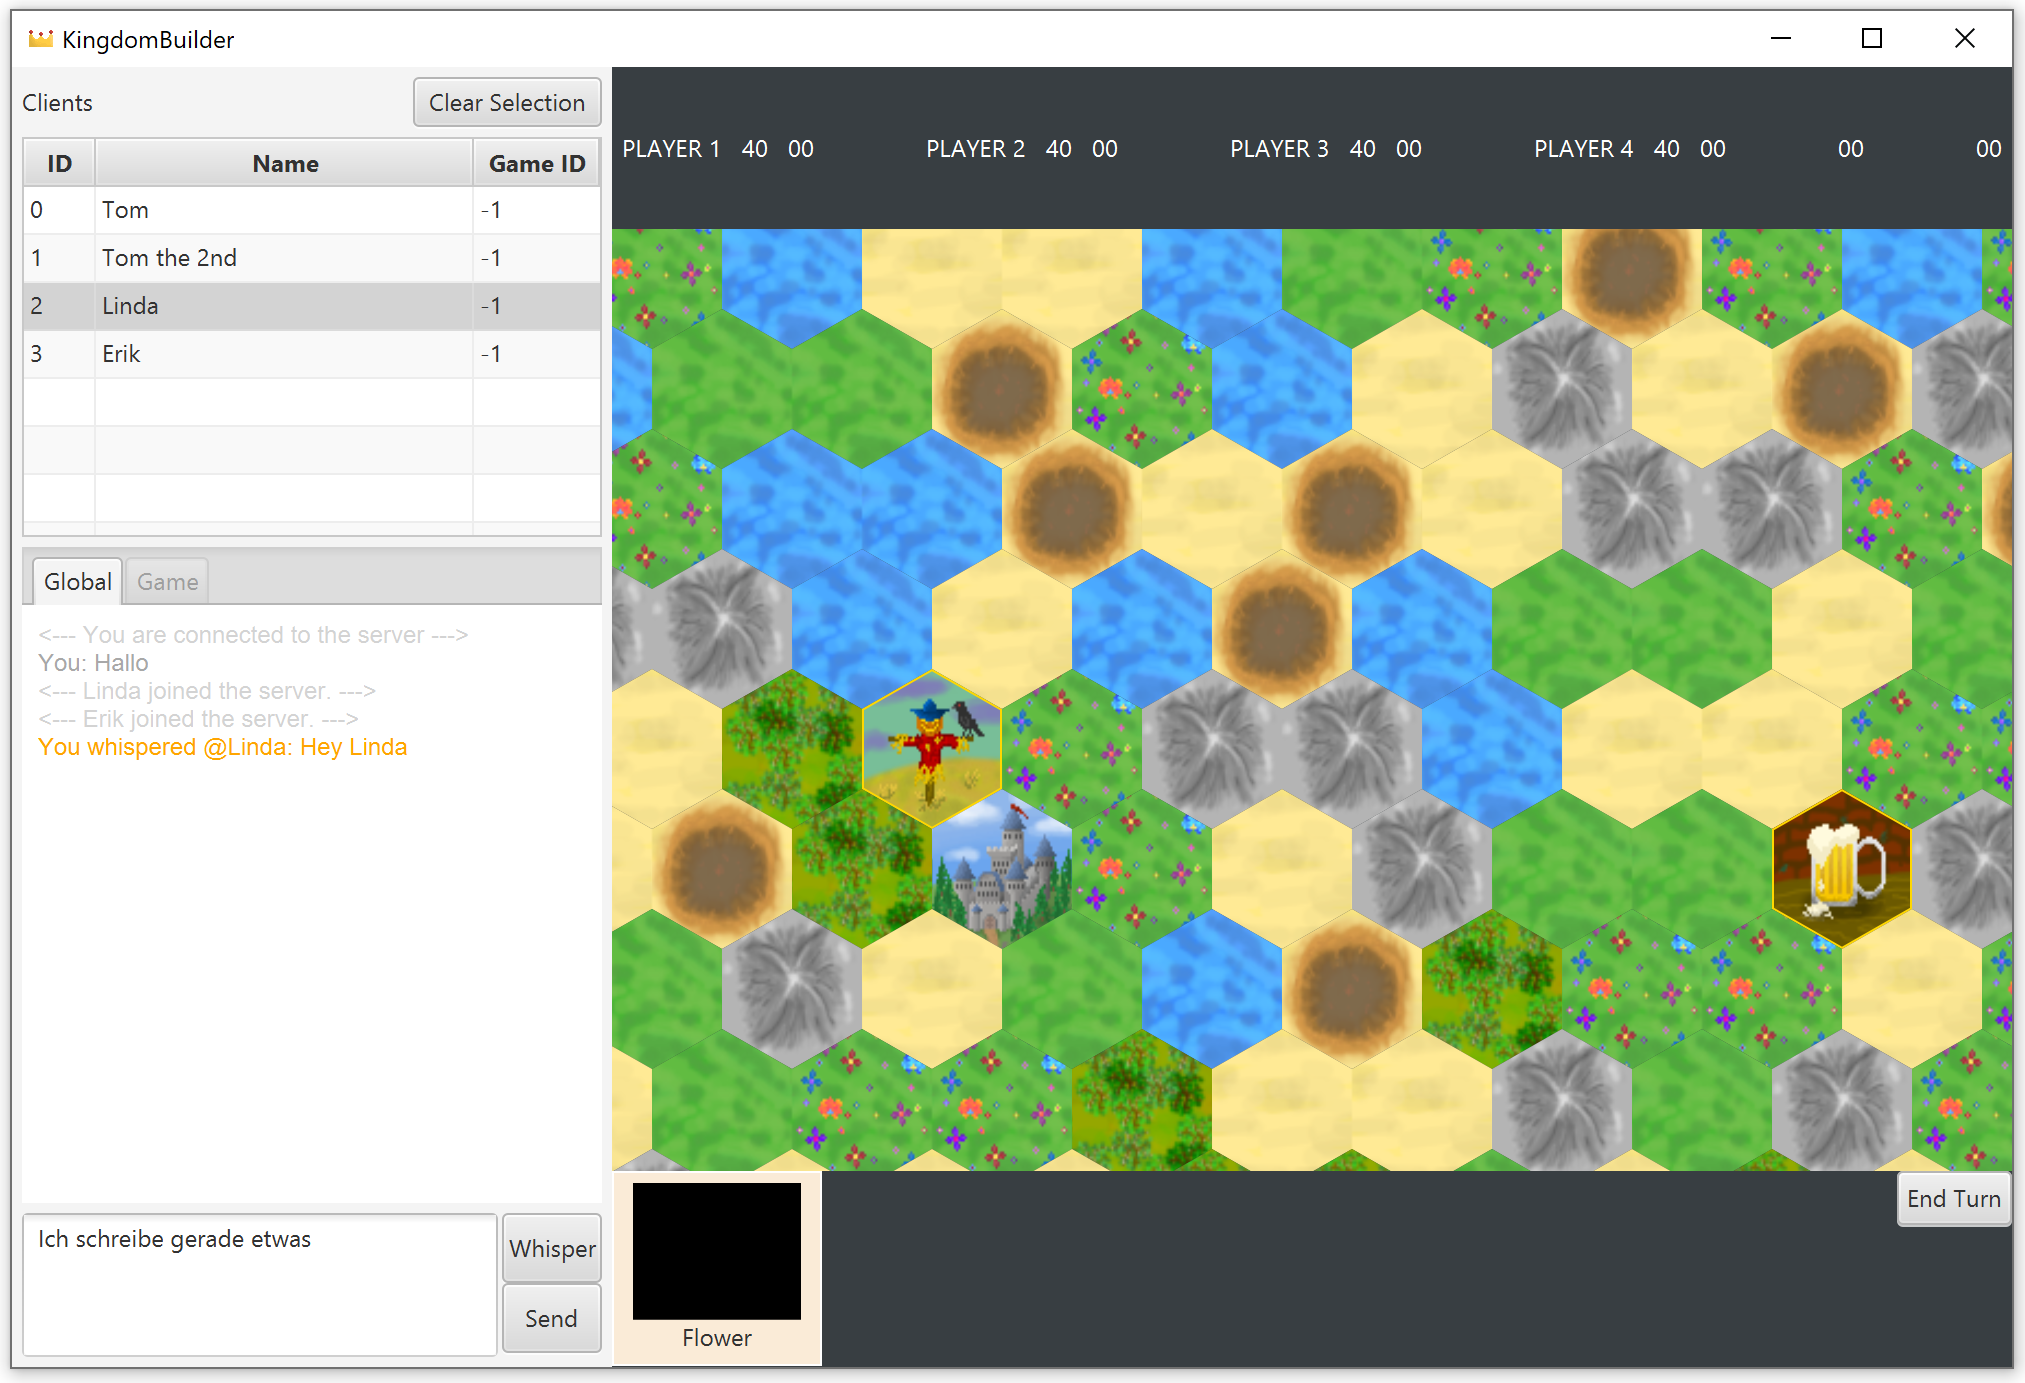
\includegraphics[width=0.8\textwidth]{view5.png}
	\\
	\tiny{(Skizze)}
\end{center}

\end{requirement}


\begin{requirement}{Spielregeln}{Hoch}{ES, BB}{16h}{-}

\begin{center}
	Als Entwickler möchte überprüfen, ob eine antizipierter Spielzug gültig ist, um fehlerhafte Züge zu unterbinden.
\end{center}

Hierbei soll eine Komponente entwickelt werden, welche anhand des aktuellen Spielfortschritts überprüft, ob der nächste Zug zulässig ist.
Ist der Zug unzulässig, so soll dieser unterbunden werden.
Die Spieler bekommen in fester Reihenfolge ihre Züge zugeteilt.
Der Ablauf eines Zuges ist aufgespalten in Basis- und Bonuszüge.
Basiszüge platzieren Siedlungen entsprechend der Feldkarte des Zuges und der benachbarten Siedlungen des Feldes, an dem die Siedlung platziert werden soll. Pro Zug müssen 3 Siedlungen auf diese Weise platziert werden.
Bonuszüge verwenden Tokens und ermöglichen es, Siedlungen zu platzieren oder zu verschieben. Jedes Token kann einmal pro Zug verwendet werden.
Ein Spieler kann einmalig von einem Token-Feld ein Token erhalten, wenn er eine Siedlung neben diesem platziert.
Es gibt 10 verschiedene Win Conditions, welche definieren, wie Punkte in einem Spiel vergeben werden. Diese werden am Anfang des Spiels festgelegt. Entsprechend der Win Conditions werden die Punkte berechnet und der Punktestand aktualisiert.


\end{requirement}


\begin{requirement}{Spielbrett 2 (GameView)}{Hoch}{TW}{10h}{2.2.7}

\begin{center}
	Als Spieler möchte ich Züge auf dem Brett ausführen können, um das Spiel zu spielen.
\end{center}

Ist auf einem Feld eine Siedlung platziert, so wird diese Siedlung auf dem Feld mit der entsprechenden Spielerfarbe gezeichnet.

Markierungen:
Zu Beginn eines Zuges werden die Hexagone markiert, auf denen eine Siedlung entsprechend des Basiszugs platziert werden kann. Wird ein Token ausgewählt, so verändern sich die Markierungen zu den Feldern, auf denen der entsprechende Token angewendet werden kann. Beim Aufheben der Token-Auswahl ändern sich die Markierungen wieder zu den zuvor markierten Feldern. Wurde der Basiszug schon getätigt, wird nichts mehr markiert.

Basiszug:
Wenn der Spieler nicht bereits alle Siedlungen für die Runde platziert hat, so kann er einen Basiszug tätigen, wobei eine Siedlung ohne Verwendung von Token platziert wird.
Wird nicht ein Token in der Schaltfläche ausgewählt und ein Hexagon des Terrain Typs der Runde angeklickt, wird geprüft, ob dies ein zulässiges Feld ist. Ist dies ein valides Feld, so wird eine Siedlung platziert. Ansonsten bekommt der Spieler eine Mitteilung, dass dies kein valides Feld ist.

Terrain Karte:
Am unteren Bildschirm befindet sich eine Anzeige, welche durch ein Bild und eine Beschreibung anzeigt, welche Terrain Karte gerade im Zug ausgewählt wurde. Diese wird jede Runde aktualisiert.

Token:
Um einen Token zu verwenden, kann dieses an der unteren Schaltfläche neben der Terrain Karte angeklickt werden. Wenn ein Token ausgewählt ist, werden andere eigene Tokens ausgegraut und deaktiviert. Dem Spieler wird anschließend durch ein Highlight gezeigt, welche Züge möglich sind und bei Bedarf können diese durchgeführt oder die Token-Auswahl abgebrochen werden, indem das Token erneut angeklickt wird.
Die Tokens werden deaktiviert, wenn der Client nicht am Zug ist. Zudem werden diese neu angezeigt, wenn sich der Hotseat Spieler wechselt.

Zum Verschieben einer Siedlung mittels Token wird die Siedlung zunächst ausgewählt und anschließend das neue Hexagon angeklickt.

Updates bei Änderungen:
Bei Zügen anderer Clients wird die Kamera der Karte zu dem Feld bewegt, bei welchem sich etwas verändert hat.


\end{requirement}



\begin{requirement}{Überarbeitung und Abschließung des Netzwerks}{Hoch}{JK, LL}{40h}{-}

\begin{center}
	Als Entwickler möchte ich alle Befehle und Benachrichtigungen des zur Verfügung gestelllten Server nutzen können.
\end{center}

Hierbei soll die Netzwerk-Komponente überarbeitet werden, so dass alle Benachrichtigungen und Befehle unterstützt werden.

\end{requirement}


\section{Meilenstein: KI und Feinschliff}


\begin{requirement}{Vollständige Integration mit dem Netzwerk-Modul}{Hoch}{JK, LL}{10h}{-}

\begin{center}
	Als Spieler möchte ich mit meinen Freunden über das Netzwerk als auch lokal am selben PC gegen KIs spielen.
\end{center}

Hierbei soll das Netzwerk-Modul umfangreich integriert werden, so dass mehrere Spieler gemeinsam über das Netzwerk an einem Spiel teilnehmen können. Hier soll auch die Möglichkeit beachtet werden, dass KIs auch als Spieler teilnehmen. Des Weiteren soll der Hot-Seat-Modus implementiert werden, so dass mehrere Spieler am selben PC gegeneinander und gegen Spieler über das Netzwerk spielen können.

\end{requirement}


\begin{requirement}{Siegesbedingung für Bots}{Hoch}{alle}{30h}{-}

\begin{center}
Ich als Entwickler möchte für Bots die Siegesbedingungen zur Verfügung stellen.
Ich als Spieler möchte meinen aktuellen Punktestand wissen.
\end{center}

Hierbei muss zwischen den 10 Siegesbedingungen unterschieden werden:
\begin{description}
	\item[Fischer] Prüft, wie viele Siedlungen angrenzend an Wasser-Feldern gebaut wurden. Pro Siedlung bekommt der Spieler, dem die Siedlung gehört, einen Punkt. Nicht beachtet werden Siedlungen, welche direkt auf Wasser liegen.
	\item[Bergleute] Prüft, wie viele Siedlungen angrenzend an Bergen gebaut wurden. Pro Berg bekommt ein Spieler einen Punkt, egal wie viele Siedlungen der Spieler an diesem Berg besitzt.
	\item[Händler] Prüft, ob ein Spieler ein oder mehrere Orts-/Burgfelder durch eigene Siedlungen verbunden hat.
	\item[Arbeiter] Prüft für jedes Orts-/Burgfeld, wie viele Siedlungen angrenzen. Pro Siedlung erhält der Spieler einen Punkt.
	\item[Entdecker] Pro Horizontaler Linie auf dem Spielbrett mit mindestens einer Siedlung bekommt der zugehörende Spieler einen Punkt.
	\item[Ritter]  Für jeden Spieler wird die horizontale Linie des Spielbretts mit seinen meisten Siedlungen ermittelt. Für jede Siedlung auf dieser Linie bekommt der Spieler 2 Punkte.
	\item[Einsiedler] Es wird 1 Punkt für jedes separate Siedlungsgebiet pro Spieler vergeben. Ein Siedlungsgebiet wird definiert durch eine Menge von angrenzenden Siedlungen.
	\item[Lords] Pro Quadrant werden Punkte vergeben. Spieler mit den meisten Siedlungen erhalten 12 Punkte. Spieler mit den zweitmeisten Siedlungen erhalten 6 Punkte.
	\item[Bürger] Jeder Spieler erhält 1 Punkt für je 2 seiner Siedlungen in seinem größten Siedlungsgebiet.
	\item[Bauern] Jeder Spieler erhält 3 Punkte für jede Siedlung in dem Quadranten, in dem er die wenigsten Siedlungen besitzt. Bei 2 Quadranten mit der gleichen geringsten Anzahl an Siedlungen wird nur ein Quadrant gewertet.

\end{description}

\end{requirement}


\begin{requirement}{Bots}{Hoch}{Alle}{20h}{2.3.2}

\begin{center}
Ich als Spieler möchte Bots zu meinem Spiel hinzufügen und somit jederzeit beliebig viele Gegenspieler für mein Spiel haben können.
\end{center}

Ermittlung strategisch günstiger Züge mittels der bereitgestellten Funktionen in der Spiellogik.

Dies erfolgt, indem mittels der Win Conditions der Zug geplant wird. Die Berechnung erfolgt in jedem Zug, da Vorausschauen nicht funktioniert, weil zukünftige Karten unbekannt sind.

Das Ziel liegt darin, den Spielzug zu optimieren und die meisten Punkte zu bekommen. Dabei werden alle möglichen platzierbaren Felder betrachtet und das beste Feld ausgesucht. In diesem Moment wird jedoch noch keine Siedlung platziert, sondern die Felder angeschaut, die nun möglich sind. Dies wird in einem Graphen aufgenommen. Hiernach werden eine oder mehrere Alternativen betrachtet, damit die KI prüft, ob die erste Siedlung wo anders platziert werden kann, damit die Punkte maximiert werden können. Alle Alternativen werden in dem Graphen aufgenommen und letztendlich der beste Zug ausgewählt und durchgeführt. Dieses Konzept ist bekannt unter dem Namen Zielorientierte Aktionsplanung (GOAP).

Die optionale Schwierigkeitseinstellung wird umgesetzt, in dem die KI für Ihre Planung für den Zug lediglich eine Teilmenge der Win Conditions auswählt. Die anspruchsvolle KI wird anhand aller Win Conditions ihren Zug planen.

Ein Bot wird mit Hilfe eines internen Client implementiert, der erstellt wird, wenn in den Spieleinstellungen ein Bot ausgewählt wird. Es wird für jeden Bot ein eigenes Client Objekt erstellt, damit dieser ein eigenen Socket zum Server besitzt und somit auch eine eigene ID. Dies ist notwendig, damit ein Bot eigene Spielzüge unabhängig vom User Client durchführen kann.

\end{requirement}


\begin{requirement}{Root}{Mittel}{tba.}{2h}{3.2.1}

\begin{center}
	Ich als Spieler möchte zum Root Spieler werden.
\end{center}

Der Chat hat eine Funktionalität, die erlaubt, mit einem Befehl “/root” und einem folgenden String als Passwort sich im Server als Root Spieler anzumelden. Die Eingabe des Befehls erfolgt im Eingabefeld für Chatnachrichten und wird bestätigt durch Absenden der Nachricht.
Nach der Anmeldung sind die folgenden administrativen Befehle des Root Spieler im Chat auf die gleiche Weise ausführbar:

Mit “/kick ID” kann ein Spieler anhand der eingegebenen ID vom Server gekickt werden.

Mit “/shutdown server” kann der Server beendet werden.

\end{requirement}


\begin{requirement}{Dekorationen}{Mittel}{tba.}{10h}{2.2.9}

\begin{center}
	Als Entwickler möchte ich eine \glqq schöne \grqq{} GUI haben um den Spieler das Spiel schmackhaft zu machen.
\end{center}

Dieses Ziel befasst sich mit dem Design der GUI. Hierbei sollen GUI-Element dekoriert und angepasst werden. Dies erfolgt unter Anderem durch die Auswahl geeigneter Farben, Schriftarten und Formen sowie Anpassungen am Layout.


\end{requirement}


\begin{requirement}{Animationen}{Gering}{tba.}{10h}{2.2.9}

Hierbei sollen Züge anschaulicher über Animationen dargestellt werden. Dabei werden insbesondere die Veränderungen am Spielbrett wie z.B. das Platzieren oder Verschieben von Siedlungen flüssig und klar verfolgbar animiert.

Optional können Wolken animiert dargestellt werden, welche sich über das Feld bewegen.

\end{requirement}


\begin{requirement}{3D-Darstellung}{Gering}{tba.}{8h}{2.2.9}

Hierbei soll das Spiel nicht mehr durch einfach 2D-Bilder sondern durch einfache 3D-Modelle dargestellt werden.

\end{requirement}

\begin{requirement}{Benutzerhandbuch}{Mittel}{alle}{10h}{2.3.5}

Erstellen eines Benutzerhandbuchs, welche dem Endanwender die Bedienung der Anwendung näher erklärt.

Der Design-Stil wird anhand unseres Programm-Stils gewählt und anschaulich mit Bildern dargestellt.

Dies wird wie im Lastenheft als Portable Document Format (pdf) in der Papiergröße DIN A5 erstellt.

\end{requirement}


\chapter{Anhang}
\section{Menüführung}
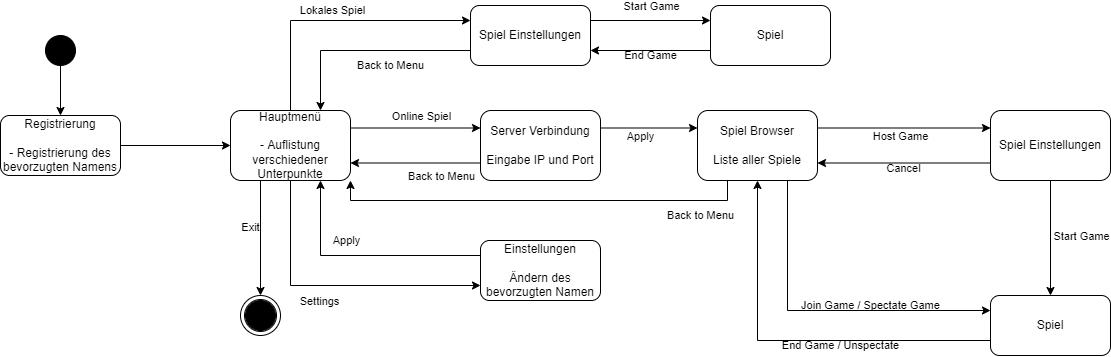
\includegraphics[width=0.8\textwidth]{menufuehrung.png}

\section{Architektur: Redux}
Die Redux Architektur besitzt verschiedene Bereiche. Es existiert der Store, mehrere Reducers, die Views und Actions.

Der Mittelpunkt ist hierbei der Store. In Redux existiert immer nur ein Store-Objekt. Dieser beinhaltet den State des ganzen Programms. Dies hat den Vorteil, dass alle Daten des Programms an einem Ort gespeichert sind und Undo und Redo Funktionen leichter umzusetzen sind. Hierbei ist jedoch zu beachten, dass Funktionen nur Leserechte auf den State haben und keine Schreibrechte.
Hier kommen die Actions in Einsatz. Interagiert der Nutzer mit der View, wird eine Action erstellt und dem Dispatcher des Stores übergeben. Dieser ruft den Reducer mit dem State und der Action auf. Nur der Reducer kann nun anhand der Action den State verändern.

Wenn der Reducer erfolgreich den State verändert hat, werden anhand der Änderung Methoden aufgerufen, die die View updaten. Dabei schreibt sich die View beim Initialisieren in eine OnChange-Methode ein und teilt dieser mit, welche Methoden aufgerufen werden müssen, wenn eine Änderung vorliegt.


\section{Glossar}
\begin{description}
	\item[Action] Objekt anhand dessen der State/Store der Application aktualisiert wird.
	\item[Application] Anwendung auf der das Spiel abläuft.
	\item[Assertion] Wird bei Tests verwendet, um einen erwarteten Wert mit einem tatsächlichen zu Vergleichen.
	\item[Basiszug] Platzieren der 3 Siedlungen auf dem gegebenen Feldtyp. Pflichtaktion pro Zug.
	\item[Benutzer] Anwender des Programms.
	\item[Bonuszug] Zusätzliche Aktion, wie Platzierung einer Siedlung auf einem vorgeschriebenen Feld oder Verschieben bereits gesetzter Siedlungen.
			     Ausgelöst werden diese durch die Verwendung von Tokens.
	\item[Bots]	Computer (Künstliche Intelligenz) die anstelle eines Menschen spielt.
	\item[Bump Map]	Verbessert den Detailreichtum von 3D Objekten.


	\item[Burgfeld]	Nicht bebaubares Feld. Bei angrenzend gebauten Siedlungen erhält der Spieler 3 Punkte.
	\item[Button] Ein Knopf, der betätigt werden kann.
	\item[Chat] Bereich in den Clients Nachrichten miteinander austauschen können.
	\item[CheckBox] Steuerelement grafischer Benutzeroberflächen. Auch bekannt als: Auswahlkasten/Kontrollkästchen/Markierungsfeld.
	\item[Client] Eine Instanz, die sich mit dem Server verbindet.
	\item[Client-Message] Message, die ein Client an den Server schickt.
	\item[ComboBox] Element der Oberfläche, mit der man unterschiedliche gegebene Eigenschaften auswählen kann.
	\item[CSS-Stylesheet] Wird für optische Verbesserungen in GUI verwendet.
	\item[Deserialisieren] Umwandlung eines Bytestroms, der durch Serialisierung eines Objekts gewonnen wurde. Der Bytestrom wird zurück in das Objekt umgewandelt.
	\item[Dialogfenster] Fehlermeldungen, die vom Server ausgegeben werden.
	\item[Direktnachricht] Schicken einer Nachricht, die nur bei einer Teilmenge an Nutzern ankommt.
	\item[Einzelspieler-Modus] Modus, in dem ein Spieler alleine spielt.
	\item[Feature] Die Funktionalität einer Software.
	\item[Fehlermeldung] Eine Benachrichtigung, wenn etwas schief geht.
	\item[Feldtyp] Typ eines Feldes (bsp.: Wüste, Wasser, Gras).
	\item[FXML Tag] Markierung, dass der folgende Code Teil ein FXML Bereich ist.
	\item[Gradle] Ist ein auf Java basiertes Build-Management-Automatisierungs-Tool. Es dient zur Beschreibung der zu bauenden Projekte.
	\item[GridPane] Layout, welche Inhalte in Tabellen Form anzeigt.
	\item[HBox] Layout, welches Inhalte nebeneinander anzeigt.
	\item[Hexagon] Ein Feld auf das ein Spieler oder Token stehen kann.
	\item[Highlight] Visuelle Darstellung bestimmter Objekte, die dadurch hervorgehoben sind.
	\item[Hosten] Erstellen eines Spiels.
	\item[Hotseat] An einem PC können mehrere Spieler gleichzeitig Spielen.
	\item[html] Hypertext Markup Language. Code welcher benötigt wird, um Webinhalte darzustellen.
	\item[ID] Eindeutige Nummer die einem Client zugeordnet wird.
	\item[Initialisieren] Das erstmalige Festlegen einer Variablen auf einen bestimmten Wert.
	\item[Interessierte / Observer / Subscriber] Methoden, die erfahren wollen, ob Veränderungen geschehen sind.
	\item[IP] Die IP des Servers an den sich der Client verbindet.
	\item[Kamera] Der bewegbare, sichtbare Ausschnitt der Karte.
	\item[Karte] Das Spielfeld für das Spiel.
	\item[KI] (Künstliche Intelligenz) Computer als nicht-menschlicher Spieler.
	\item[Kicken] Einen Client vom Server trennen.
	\item[Label] Ein GUI Element, welches Text anzeigt.
	\item[Leserecht] Liest nur Daten und kann diese nicht modifizieren.
	\item[Markierung] Visuelle Darstellung bestimmter Objekte, die dadurch hervorgehoben sind.
	\item[modular] Ein ganzer Block aufgeteilt in kleinere Module, Komponenten oder Bausteine.
	\item[Netzwerknachricht] Eine Nachricht, wenn der Server eine Message an den Client sendet.
	\item[Ortsfeld] Unbebaubare Felder. Angrenzende Siedlungen bekommen einen Token.
	\item[Parsen] Zerlegung und Umwandlung einer Eingabe in ein für die Weiterverarbeitung geeigneteres Format.
	\item[Protokoll] Gegebenes Server-Protokoll, in dem jede Server-/Client-Message aufgeführt ist.
    \item[Port] Adresse am Server an der sich ein Client verbinden kann.
    \item[Quadrant] Das Spielfeld wird in vier Teile aufgeteilt. Ein Quadrant ist eines davon.
    \item[quittieren] Synonym für beenden.
    \item[Record(-Datentyp)] Spezielle Klasse zur Speicherung unveränderlicher Daten, wobei Accessor-Methoden, hashCode(), toString() und equals() implizit implementiert sind.
    \item[Rectangle] Java FX Klasse für Rechtecke.
    \item[Redo] Etwas wiederholen.
    \item[Reducer] Teil der Redux Architektur. Ist zuständig, die durch Actions aufgerufenen Änderungen am State durchzuführen.
    \item[rendern] Zeichnen und Anzeigen einer Grafik.
    \item[Repository] Stellt ein verwaltetes digitales Verzeichnis zur Speicherung digitaler Objekte dar.
    \item[Root Spieler] Benutzer mit administrativen Rechten.
    \item[Schreibrecht] Kann Daten lesen und modifizieren.
    \item[Server] Repräsentiert ein Computerprogramm oder ein Gerät, welches Daten, Funktionalitäten oder Dienstprogramme bereitstellt, damit andere Computer oder Programme darauf zugreifen können. Dies geschieht meist über ein Netzwerk.
    \item[Server-Message] Eine Nachricht, die vom Server gesendet wird und Informationen für Clients enthält.
    \item[Siedlung] Die Spielfigur des Spieles, welche auf ein Hexagon platziert werden kann.
    \item[Siedlung platzieren] Eine Spielfigur auf einem Feld platzieren.
    \item[Siedlung verschieben] Eine Spielfigur von einem Feld entfernen und auf ein anderes Feld platzieren.
    \item[Siedlungsfelder] Felder auf dem Spielbrett, welche mit einer Siedlung bebaut sind.
	\item[Sieges-Karten / Siegesbedingungen] Drei von zehn ausgewählten Siegesbedingungen. Diese beschreiben, unter welchen Bedingungen ein Spieler Punkte bekommt.
	    \item[Snake-Case] Notation von Variablen mit Unterstrichen.
	    \item[Spiel beitreten] Ein Benutzer tritt einem Spiel bei, um in diesem zu spielen oder diesem zuzuschauen.
	    \item[Spielbrett] Das Spielfeld, das aus den 4 Quadranten beziehungsweise deren einzelnen Feldern besteht.
	    \item[Spielfunktion] Die Funktionen, die benötigt werden, ein Spiel als Datenstruktur zu verwalten.
	    \item[Spielerfarbe] Die eindeutige Farbe, die einem Spieler am Anfang des Spiel zugeordnet wird.
	    \item[Spielstatus] Der Status eines Spiels. Ein Spiel kann auf Spieler warten, gestartet sein und laufen oder beendet sein.
	    \item[Spielzug] Ein Zug eines Spielers in einem Spiel. Dieser besteht aus Pflichtaktionen wie dem Basiszug und optionalen Aktionen wie dem Spielen von Tokens.
	    \item[State] Teil der Redux Architektur. Die State speichert die Daten des Programms.
	    \item[Store] Teil der Redux Architektur. Der Store bildet die Schnittstelle zur State.
	    \item[SubScene] Eine abstrahierte Teilmenge der gesamten Szene, um nur bestimmte Daten zu lesen.
	    \item[subscribe] Sich als Teilprogramm einschreiben, um benachrichtigt zu werden, wenn ein Kriterium erfüllt ist.
	    \item[Subscriber] Ein Teilprogramm, welches benachrichtigt wird, wenn ein Kriterium erfüllt ist.
	    \item[Substate] Teil der Redux Architektur. Einzelne Unterkategorien der State, welchen separat subscribed werden kann.
	\item[Socket] Die lokale Anbindung der direkten Verbindung zum Server.
	\item[SpinBox] Element der Oberfläche, mit welchem eine Zahl spezifiziert werden kann.
	\item[Szene] Die Benutzeroberfläche, welche im Fenster angezeigt wird.
	\item[Tab] Element, welches eine Registerkarte darstellt.
	\item[TableView] Element, welches eine Tabelle anzeigt.
	\item[Terrain Karte] Element der Oberfläche, welches das gegebene Terrain der Runde anzeigt in Form eines Bildes und einer Beschreibung.
	\item[Terrain Typ] Bebaubaren Feldtypen wie Gras, Blumen etc.
	\item[TextArea] Element der Oberfläche, welches Text anzeigt.
	\item[TextField] Element der Benutzeroberfläche, welches erlaubt, eine Texteingabe zu tätigen.
	\item[Textur] Darstellung von Spielobjekte als Bilder (bsp.: Gras oder Settlement).
	\item[Tile] Ein Feld bzw. einzelnes Hexagon der Spielkarte.
	\item[Token] Ein Ortsplättchen, welche dem Spieler ermöglicht, Bonuszüge zu tätigen.
	\item[Token-Typ] Die Art des Token die man erhalten kann, wenn man auf einen besonderen Ort anbaut.
	\item[Undo] Etwas Rückgängig machen.
	\item[User] Anwender des Programms.
	\item[WebView] Darstellung des Chatfensters in HTML.
	\item[Win Conditions] Drei von zehn ausgewählten Siegesbedingungen. Diese beschreiben, unter welchen Bedingungen ein Spieler Punkte bekommt.
	\item[Zeitlimit] Zeitbegrenzung für eine Runde in einem Spiel.
	\item[Zoom] Karte vergrößern oder verkleinern.
	\item[Zug] Erste bis letzte Aktion während ein Spieler dran ist.
	\item[Zug beenden] Beendet seinen Zug, wenn die Pflichtaktion der 3 Siedlungen abgeschlossen ist und überspringt die Verwendung von Tokens.
	\item[Zuglimit] Maximale Anzahl an Runden in einem Spiel.
\end{description}


\end{document}
